\chapter{Libnodegit}

This section aims to give a detailed view into some important concepts and
implementation details.

\begin{figure}[htb]
  \centering
  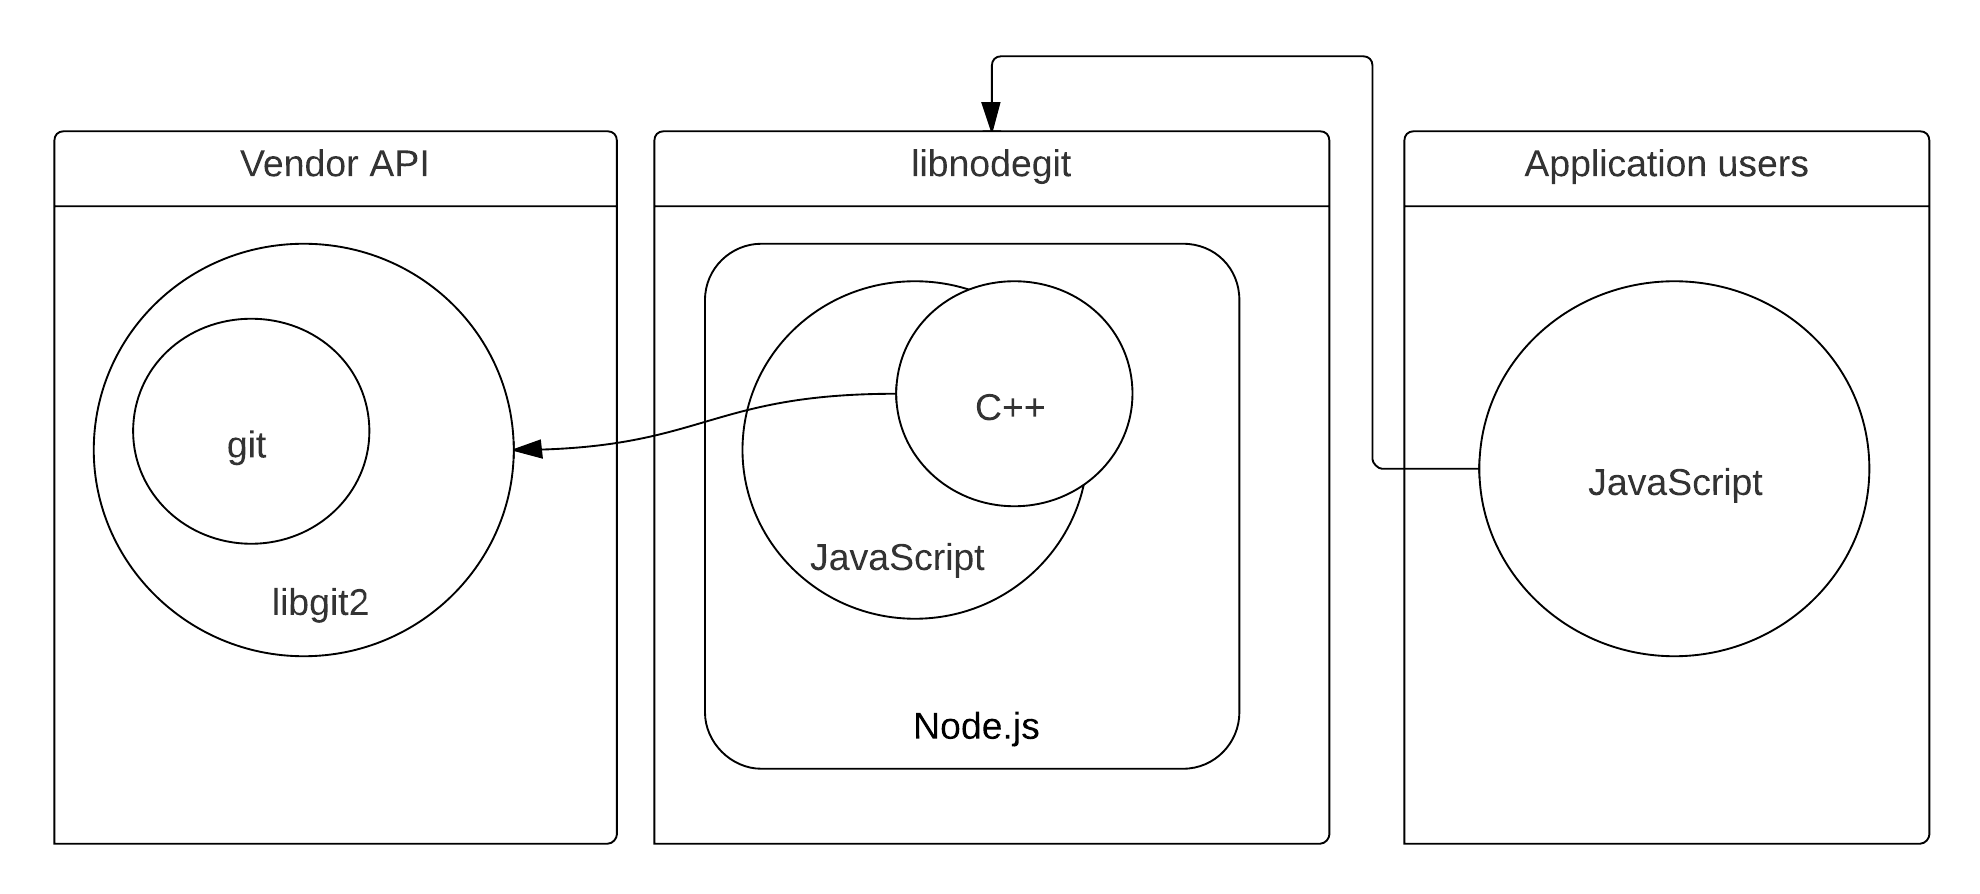
\includegraphics[scale=0.27]{./diagrams/architecture.png}
  \caption{Libnodegit architecture}
  \label{fig:architecture}
\end{figure}

\section{Design as  decisions}

If the same task can be done with both C++ and JavaScript, which language should
be used to do that? This was probably one of the hardest design decisions in the
entire project, went through several iterations and finally the decision was to
do it with JavaScript. The final version of the project is the result of so many
such decisions, and a few will be discussed here.

The original idea was to do it with C++. Implementing the logic in one place
will reduce complexity and maintenance overhead. This turned out to be very
difficult and the idea was dropped for the alternative. A few such decisions
are,

\subsection{Polish API with JS wrapper functions}

Almost all functions implemented in C++, end with a trailing underscore, like
\texttt{reference\_}, \texttt{head\_} etc and is almost never exposed from the
API. An equivalent wrapper function in JavaScript will be called
\texttt{reference} or \texttt{head} respectively. Wrapper functions will use the
underlying C++ implementation and return data appropriately. \\

\textbf{Pros:}
\begin{enumerate}

	\item Doing the same task almost always require less code in JavaScript.
    \item Programming JavaScript is generally easier.
    \item Wrapper functions make lazy evaluation easier.
    \item Argument validation can be much faster with JavaScript. For eg, if function
      expects \texttt{n} arguments, an exception is thrown at JavaScript wrapper
      before dropping down to C++ if it gets less than n arguments.
    \item Return types can be modified with JavaScript easily.

\end{enumerate}

\textbf{Cons:}
\begin{enumerate}

	\item Often the same application logic is split between functions written in 2
      very different languages, making maintenance difficult.

\end{enumerate}

\subsection{Prefer lazy evaluation wherever possible}

Wrapper functions can be used for performance gain with lazy evaluation. For
example, the C++ function \texttt{parents\_} return an array of SHA1 strings,
and the wrapper function \texttt{parents} converts it into an array of reference
instances only when the function is explicitly called, and not when the original
commit instance is constructed.

\subsection{Automate tasks with tests and build tools like gyp/Makefiles}

Ease of inclusion of this library in a 3rd party module is critically important
for its adaptation and success. Generally node.js libraries can be pushed to the
NPM\cite{npm} repository so that other developers can install it with one single
command, \texttt{npm install libnodegit}.

The complexity of the project makes it hard to do so, but it is possible. This
will be a priority and can be achieved only with maximum automation.

\section{API}

The API is essentially is an interface abstracting the low level \texttt{git
  --plumping} or \texttt{libgit2} to a higher level. It is explained with
examples.

\subsection{API example - \texttt{git log}}

The simplest of the git operations is to see the log of the project history.
Here is an example of getting the details of the last 3 commits from the
libnodegit project the normal git way.

\begin{verbatim}

$ cd Projects/libnodegit/
$ git log -3

commit 1a9973aacc3a080add250228a9cee571945e72ec
Author: Jaseem Abid <jaseemabid@gmail.com>
Date:   Fri Apr 26 19:23:21 2013 +0530

    README fixes

commit 0dd1b45b20a1e4827d268f1b859ffcb5dd39069d
Author: Jaseem Abid <jaseemabid@gmail.com>
Date:   Sat Apr 20 07:37:04 2013 +0530

    `npm link` loops calling npm rebuild

    This might be the issue, deal later.
    https://github.com/isaacs/npm/issues/2788

commit 01b58820ae28938dec9bb5575afc4624a992b21d
Author: Jaseem Abid <jaseemabid@gmail.com>
Date:   Mon Mar 25 21:15:30 2013 +0530

    Whitespace fixes

\end{verbatim}

Its quite easy and convenient for humans to parse this output and get the
required information out of it. Consider parsing this for machine consumption.
Getting a list of SHA1 ids or emails out of this takes us back to regular
expressions and language parsers - an overhead and error prone task. This is
what libnodegit is trying to improve.

Here is the same task with libnodegit library.

\begin{verbatim}

# Require the library
l = require "libnodegit"

# Initialize the repo with path alone
repo = new l.Repository "~/Projects/libnodegit"

# Get last 2 commits
commits = repo.log {count : 2}

# Print the commits array
console.log commits

// Commits array
[
    {
      "commit": "1a9973aacc3a080add250228a9cee571945e72ec",
      "author": {
        "name": "Jaseem Abid",
        "email": "jaseemabid@gmail.com"
      },
      "date": "Fri Apr 26 19:23:21 2013 +0530",
      "message": "README fixes"
    },
    {
      "commit": "0dd1b45b20a1e4827d268f1b859ffcb5dd39069d",
      "author ": {
        "name": "Jaseem Abid",
        "email": "jaseemabid@gmail.com>"
      },
      "date": "Sat Apr 20 07:37:04 2013 +0530",
      "message": "`npm link` loops calling npm rebuild''
    }
]

\end{verbatim}

In the example, the log function returns an array of commit objects, each with
its own properties which can be easily manipulated and required information can
be easily filtered from it. Extracting the list of SHA ids is a trivial task
here.
